\chapter{Titrations by pH and Conductivity}\label{ch:g12:ph-conductivity-titrations}

A bottle of wine vinegar is labelled ``6 \% acidity'': six grams of
ethanoic acid in every hundred grams of vinegar. Neither ethanoic acid
nor its conjugate base is coloured, and no permanganate will help here.
But a \omterm{def:g9:acids-bases-ph:ph-paper}{pH meter} dipped into the vinegar, or a cell measuring how well it
conducts, follows the reaction with a base drop by drop, and the shape
of the curve shows exactly where \omterm{def:g11:titration:equivalence}{equivalence} lies. Ten minutes at the
bench, and the label is checked.

\begin{recall}
A \omterm{def:g11:titration:titration}{titration}, its \omterm{def:g11:titration:equivalence}{equivalence} and \omterm{def:g11:titration:equivalence}{equivalent volume}
(\cref{ch:g11:titration}); \omterm{def:g12:ka-and-pka:ka}{acidity constants} (\cref{ch:g12:ka-and-pka});
Henderson's relation and indicators
(\cref{ch:g12:buffers-predominance}); solutions of \omterm{def:g9:ions:ion}{ions} conduct
electricity (\cref{ch:g9:ions}).
\end{recall}

\begin{omfigure}
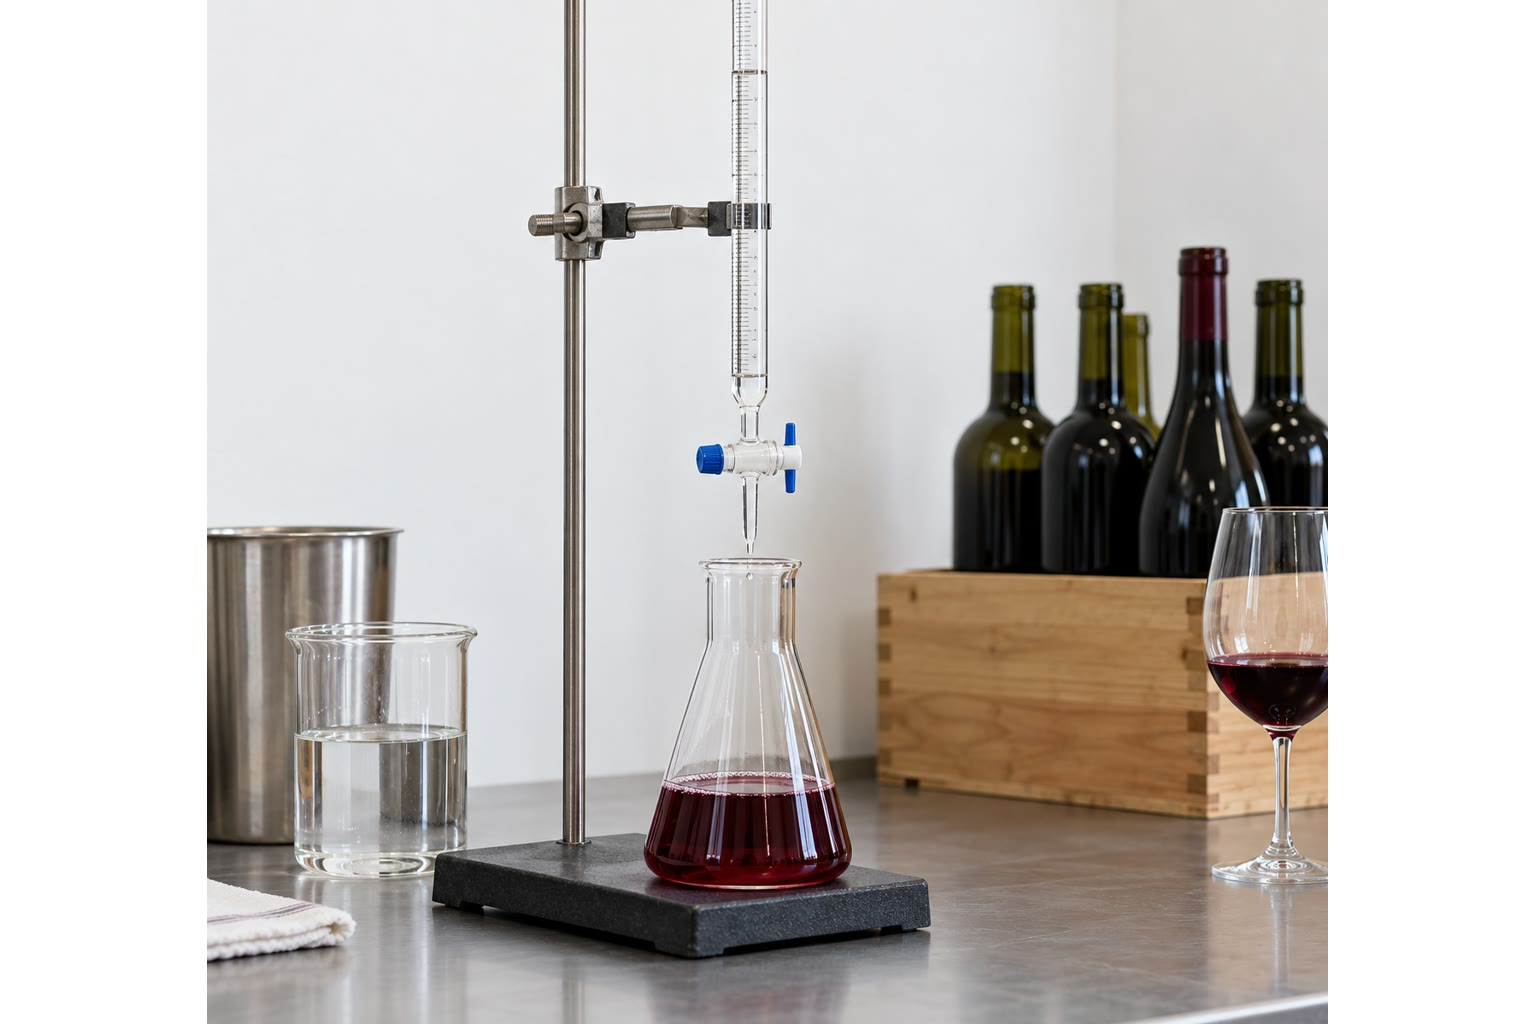
\includegraphics[width=0.45\linewidth]{images/book1/ai/g12-wine-lab.jpg}

{\small A wine-maker's \omterm{def:g11:titration:titration}{titration} bench.}
\end{omfigure}

\section{The pH-metric titration}

\begin{definition}[pH-metric titration, half-equivalence]\label{def:g12:ph-conductivity-titrations:ph-metric}
In a \emph{pH-metric titration}\index{pH-metric titration} the \omterm{def:g9:acids-bases-ph:ph}{pH} of the
\omterm{def:g11:titration:titration}{titrated solution} is measured after each addition of \omterm{def:g11:titration:titration}{titrant}, and the
curve \omterm{def:g9:acids-bases-ph:ph}{pH} against the volume added is drawn. \emph{Half-equivalence}\index{half-equivalence}
is the point where half the \omterm{def:g11:titration:equivalence}{equivalent volume} has been added.
\end{definition}

\begin{omfigure}
\begin{tikzpicture}[font=\small, scale=0.65]
  \pic[transform shape] at (0,0) {stand={6.3}{2.0}};
  \pic[transform shape] at (2.0,0.68) {stirrer};
  \pic[transform shape] at (2.0,0.68) {beaker={0.45}{omWater}};
  \pic[transform shape] at (2.0,2.9) {burette={0.8}{omWater}};
  \pic[transform shape] (pr) at (2.6,0.95) {probe};
  \pic[transform shape] (m) at (6.4,3.4) {meter={pH}};
  \draw[black!70, thick] (pr-top) .. controls +(0,1.0) and +(0,-1.2) .. (m-a);
  \draw[omProp, thick, <-] (2.35,7.2) -- (4.3,7.6) node[right, text=black] {burette: NaOH};
  \draw[omProp, thick, <-] (1.4,1.1) -- (-1.4,1.6) node[left, text=black, align=right] {acid to titrate};
  \draw[omProp, thick, <-] (2.75,2.4) -- (4.3,2.0) node[right, text=black] {pH probe};
\end{tikzpicture}

{\small A \omterm{def:g12:ph-conductivity-titrations:ph-metric}{pH-metric titration}: the probe dips in the stirred solution,
the meter shows the \omterm{def:g9:acids-bases-ph:ph}{pH} after each addition.}
\end{omfigure}

\begin{inthelab}[Calibrating a pH meter]
Before use, the probe is rinsed with distilled water and dipped in two
\omterm{def:g12:buffers-predominance:buffer}{buffer solutions} of known \omterm{def:g9:acids-bases-ph:ph}{pH}, usually 7.0 and 4.0 (or 10.0): the meter
is set to read their values. Between solutions the probe is rinsed and
gently dabbed dry, never wiped; it is stored with its tip wet.
\end{inthelab}

\begin{omfigure}
\begin{minipage}{0.49\linewidth}
\begin{tikzpicture}
\begin{axis}[width=\linewidth, height=6cm, xmin=0, xmax=30, ymin=0, ymax=14,
    xlabel={$V_{\text{NaOH}}$ (\si{mL})}, ylabel={pH}, axis lines*=left,
    ymajorgrids, grid style={gray!20}, tick label style={font=\scriptsize},
    label style={font=\small}, title={\small \ce{HCl} by \ce{NaOH}},
    title style={yshift=-4pt}]
  \addplot[very thick, omDef] table[x=V, y=pH] {figdata/out/grade-12-ph-conductivity-titrations-a.dat};
  \addplot[thick, omProp, densely dotted] table[x=V, y expr=\thisrow{dpH}/4]
    {figdata/out/grade-12-ph-conductivity-titrations-a.dat};
  \addplot[dashed, black!60] coordinates {(20,0) (20,7)};
  \node[font=\scriptsize, anchor=north west] at (axis cs:20.3,6.5) {$V_E = 20.0$};
\end{axis}
\end{tikzpicture}
\end{minipage}\hfill
\begin{minipage}{0.49\linewidth}
\begin{tikzpicture}
\begin{axis}[width=\linewidth, height=6cm, xmin=0, xmax=16, ymin=0, ymax=14,
    xlabel={$V_{\text{NaOH}}$ (\si{mL})}, ylabel={pH}, axis lines*=left,
    ymajorgrids, grid style={gray!20}, tick label style={font=\scriptsize},
    label style={font=\small}, title={\small \ce{CH3COOH} by \ce{NaOH}},
    title style={yshift=-4pt}]
  \addplot[very thick, omDef] table[x=V, y=pH] {figdata/out/grade-12-ph-conductivity-titrations-b.dat};
  \addplot[thick, omProp, densely dotted] table[x=V, y expr=\thisrow{dpH}/4]
    {figdata/out/grade-12-ph-conductivity-titrations-b.dat};
  \addplot[dashed, black!60] coordinates {(10.1,0) (10.1,8.7)};
  \addplot[dashed, black!60] coordinates {(0,4.76) (5.05,4.76) (5.05,0)};
  \node[font=\scriptsize, anchor=south west] at (axis cs:0.2,4.8) {$pK_a = 4.76$};
  \node[font=\scriptsize, anchor=north west] at (axis cs:10.4,3.0) {$V_E = 10.1$};
\end{axis}
\end{tikzpicture}
\end{minipage}

{\small Computed \omterm{def:g9:acids-bases-ph:ph}{pH} curves (blue) and their derivative $d\mathrm{pH}/dV$
(orange, dotted, divided by 4). Left: \qty{20.0}{mL} of hydrochloric acid
at \qty{0.100}{mol/L}; \omterm{def:g11:titration:equivalence}{equivalence} at \omterm{def:g9:acids-bases-ph:ph}{pH} 7.00. Right: \qty{10.0}{mL} of
diluted vinegar; at \omterm{def:g12:ph-conductivity-titrations:ph-metric}{half-equivalence} the \omterm{def:g9:acids-bases-ph:ph}{pH} equals the $pK_a$, and
\omterm{def:g11:titration:equivalence}{equivalence} lies at a basic \omterm{def:g9:acids-bases-ph:ph}{pH}.}
\end{omfigure}


\begin{method}[The derivative method]\label{met:g12:ph-conductivity-titrations:derivative}
Compute, between successive measurements, the slope
$\Delta\mathrm{pH}/\Delta V$, and plot it against $V$ (a spreadsheet or a
calculator does it). The \omterm{def:g11:titration:equivalence}{equivalent volume} is where this slope is
largest: the peak of the derivative curve.
\end{method}

\begin{method}[The tangent method]\label{met:g12:ph-conductivity-titrations:tangent}
\begin{enumerate}
  \item Draw two parallel tangents to the curve, one before and one after
        the jump, on either side of it.
  \item Draw the parallel line halfway between them.
  \item Where it cuts the curve is the \omterm{def:g11:titration:equivalence}{equivalence} point: read $V_E$ (and
        the \omterm{def:g9:acids-bases-ph:ph}{pH} at \omterm{def:g11:titration:equivalence}{equivalence}).
\end{enumerate}
\end{method}

\begin{proposition}[At half-equivalence, $\mathrm{pH} = pK_a$]\label{prop:g12:ph-conductivity-titrations:half}
In the \omterm{def:g11:titration:titration}{titration} of a \omterm{def:g12:ka-and-pka:strong-acid}{weak acid} \ce{HA} by a \omterm{def:g12:ka-and-pka:strong-acid}{strong base}, at
\omterm{def:g12:ph-conductivity-titrations:ph-metric}{half-equivalence} $\mathrm{pH} = pK_a$.
\end{proposition}

\begin{proof}
The reaction \ce{HA + OH- -> A- + H2O} is total. At \omterm{def:g12:ph-conductivity-titrations:ph-metric}{half-equivalence} half
of the acid has been turned into \ce{A-}: $[\ce{A-}] = [\ce{HA}]$, and
Henderson's relation gives $\mathrm{pH} = pK_a + \log 1 = pK_a$.
\end{proof}

\begin{remark}[Choosing an indicator from the curve]\label{rem:g12:ph-conductivity-titrations:indicator}
% ledger: ind:BBT, ind:phenolphthalein
The indicator must change colour inside the jump. For hydrochloric acid
the jump spans about \omterm{def:g9:acids-bases-ph:ph}{pH} 4 to 10 and many indicators fit, bromothymol blue
best; for ethanoic acid the jump is shorter and basic, around 7 to 11:
phenolphthalein (8.0--10.0) fits, bromothymol blue would change too
early.
\end{remark}

\section{Conductivity and conductimetric titrations}

\begin{definition}[Conductivity, molar ionic conductivity]\label{def:g12:ph-conductivity-titrations:conductivity}
The \emph{conductivity}\index{conductivity} $\sigma$ of a solution
measures how well it conducts electricity; it is read on a conductimeter
in \si{mS/cm} (or \si{S/m}). Each \omterm{def:g9:ions:ion}{ion} $i$ contributes to it in
proportion to its concentration, with a coefficient $\lambda_i$, its
\emph{molar ionic conductivity}\index{molar ionic conductivity}.
\end{definition}

\begin{proposition}[Kohlrausch's law]\label{prop:g12:ph-conductivity-titrations:kohlrausch}
% ledger: lam:H+, lam:OH-, lam:Na+, lam:Cl-
For a dilute solution, $\sigma = \sum_i \lambda_i [X_i]$. At
\qty{25}{\celsius}, in \si{S.cm^2/mol}: \ce{H3O+} 349.8, \ce{OH-} 198.3,
\ce{Cl-} 76.2, \ce{Na+} 50.3. The oxonium and hydroxide \omterm{def:g9:ions:ion}{ions} conduct far
better than all other \omterm{def:g9:ions:ion}{ions}.
\end{proposition}

\begin{proof}
Admitted (Year 1 volume). The values of \ce{Cl-} and \ce{Na+} come from
the measured conductivities of hydrochloric acid and sodium chloride
solutions, from which that of \ce{H3O+} is subtracted.
\end{proof}

\begin{definition}[Conductimetric titration]\label{def:g12:ph-conductivity-titrations:conductimetric}
In a \emph{conductimetric titration}\index{conductimetric titration} the
\omterm{def:g12:ph-conductivity-titrations:conductivity}{conductivity} is measured after each addition of \omterm{def:g11:titration:titration}{titrant}. The \omterm{def:g11:titration:titration}{titrated
solution} is diluted in a large volume of water, so that the volume
added hardly changes it: the points then lie on straight lines, which
change slope at \omterm{def:g11:titration:equivalence}{equivalence}.
\end{definition}

\begin{omfigure}
\begin{minipage}{0.4\linewidth}\centering
\begin{tikzpicture}[font=\small, scale=0.75]
  \pic[transform shape] at (0,0) {beaker={0.6}{omWater}};
  \pic[transform shape] (cc) at (0.2,0.2) {condcell};
  \pic[transform shape] (m) at (2.6,3.4) {meter={mS/cm}};
  \draw[black!70, thick] (cc-top) .. controls +(0,0.8) and +(0,-1) .. (m-a);
  \node[anchor=north, align=center] at (0.6,-0.15) {conductimetry cell\\ in the solution};
\end{tikzpicture}
\end{minipage}\hfill
\begin{minipage}{0.56\linewidth}
\begin{tikzpicture}
\begin{axis}[width=\linewidth, height=5.4cm, xmin=0, xmax=20, ymin=0,
    ymax=4.6, xlabel={$V_{\text{NaOH}}$ (\si{mL})}, ylabel={$\sigma$ (\si{mS/cm})},
    axis lines*=left, ymajorgrids, grid style={gray!20},
    tick label style={font=\scriptsize}, label style={font=\small}]
  \addplot[only marks, mark=*, mark size=1.4pt, omDef] table[x=V, y=sigma]
    {figdata/out/grade-12-ph-conductivity-titrations-c.dat};
  \addplot[dashed, black!60] coordinates {(10,0) (10,4.6)};
  \node[font=\scriptsize, anchor=south west] at (axis cs:10.3,0.2) {$V_E = 10.0$};
\end{axis}
\end{tikzpicture}
\end{minipage}

{\small Left: a conductimetry cell. Right: \qty{100}{mL} of hydrochloric
acid at \qty{0.0100}{mol/L} titrated by sodium hydroxide at
\qty{0.100}{mol/L} (computed with Kohlrausch's law). The \omterm{def:g12:ph-conductivity-titrations:conductivity}{conductivity}
falls, then rises: two straight lines meeting at \omterm{def:g11:titration:equivalence}{equivalence}.}
\end{omfigure}

\begin{example}[Reading the two lines]\label{ex:g12:ph-conductivity-titrations:lines}
Before \omterm{def:g11:titration:equivalence}{equivalence} each \ce{OH-} added removes an \ce{H3O+}
($\lambda = 349.8$) and brings in a \ce{Na+} ($\lambda = 50.3$): the
\omterm{def:g12:ph-conductivity-titrations:conductivity}{conductivity} falls steeply. After \omterm{def:g11:titration:equivalence}{equivalence}, \ce{Na+} and \ce{OH-}
($\lambda = 198.3$) simply accumulate: it rises. The two lines meet at
$V_E = \qty{10.0}{mL}$, so the acid was
$0.100 \times 10.0 / 100 = \qty{0.0100}{mol/L}$.
\end{example}

\begin{method}[Equivalence from a conductimetric titration]\label{met:g12:ph-conductivity-titrations:two-lines}
Draw the best straight line through the points before \omterm{def:g11:titration:equivalence}{equivalence} and
the best line through the points after it; read $V_E$ at their
intersection. Points near \omterm{def:g11:titration:equivalence}{equivalence}, where the lines bend, are left
out.
\end{method}

\begin{remark}[Which method when]\label{rem:g12:ph-conductivity-titrations:which}
A coloured indicator is fastest when a suitable one exists. A \omterm{def:g12:ph-conductivity-titrations:ph-metric}{pH-metric
titration} also gives the $pK_a$ of a \omterm{def:g12:ka-and-pka:strong-acid}{weak acid}, and works with coloured
or cloudy solutions. A \omterm{def:g12:ph-conductivity-titrations:conductimetric}{conductimetric titration} needs no jump in \omterm{def:g9:acids-bases-ph:ph}{pH} at
all: it works for very weak or very dilute acids, and for \omterm{def:g9:ions:precipitate}{precipitation}
reactions, as long as the \omterm{def:g9:ions:ion}{ions} change.
\end{remark}

\begin{safety}{\ghs[0.82cm]{GHS05}\ghs[0.82cm]{GHS07}}
% ledger: ghs:NaOH
Sodium hydroxide solutions burn the skin and the eyes, even dilute ones
in the eyes: goggles throughout, and any splash rinsed at once with a
lot of water.
\end{safety}

\section{Exercises}


\begin{exercise}[$\star$]\label{exo:g12:ph-conductivity-titrations:1}
Read the \omterm{def:g11:titration:equivalence}{equivalent volume} on the curve of hydrochloric acid titrated by
sodium hydroxide at \qty{0.100}{mol/L}, and deduce the concentration of
the \qty{20.0}{mL} of acid.
\end{exercise}

\begin{exercise}[$\star$]\label{exo:g12:ph-conductivity-titrations:2}
A \omterm{def:g12:ka-and-pka:strong-acid}{weak acid} is titrated by sodium hydroxide; $V_E = \qty{12.0}{mL}$. At
\qty{6.0}{mL} the \omterm{def:g9:acids-bases-ph:ph}{pH} is 3.75. Give the $pK_a$ of the acid. Which acid of
the $pK_a$ scale could it be?
\end{exercise}

\begin{exercise}[$\star$]\label{exo:g12:ph-conductivity-titrations:3}
Which indicator would you choose for the \omterm{def:g11:titration:titration}{titration} of ethanoic acid by
sodium hydroxide? Why not methyl red?
\end{exercise}

\begin{exercise}[$\star$]\label{exo:g12:ph-conductivity-titrations:4}
Why must a \omterm{def:g9:acids-bases-ph:ph-paper}{pH meter} be calibrated before use? With what?
\end{exercise}

\begin{exercise}[$\star$]\label{exo:g12:ph-conductivity-titrations:5}
Using the molar ionic conductivities, rank the \omterm{def:g9:ions:ion}{ions} \ce{H3O+}, \ce{OH-},
\ce{Na+}, \ce{Cl-} from the best conductor to the worst.
\end{exercise}

\begin{exercise}[$\star\star$]\label{exo:g12:ph-conductivity-titrations:6}
\qty{20.0}{mL} of an ethanoic acid solution need \qty{14.6}{mL} of
sodium hydroxide at \qty{0.050}{mol/L}. Compute its concentration.
\end{exercise}

\begin{exercise}[$\star\star$]\label{exo:g12:ph-conductivity-titrations:7}
Near \omterm{def:g11:titration:equivalence}{equivalence}, the readings are: \qty{9.6}{mL}, \omterm{def:g9:acids-bases-ph:ph}{pH} 5.7;
\qty{9.8}{mL}, 6.1; \qty{10.0}{mL}, 7.0; \qty{10.2}{mL}, 10.5;
\qty{10.4}{mL}, 11.0. Compute $\Delta\mathrm{pH}/\Delta V$ between
successive points and locate $V_E$.
\end{exercise}

\begin{exercise}[$\star\star$]\label{exo:g12:ph-conductivity-titrations:8}
In the \omterm{def:g12:ph-conductivity-titrations:conductimetric}{conductimetric titration} of hydrochloric acid, explain the sign of
the slope before \omterm{def:g11:titration:equivalence}{equivalence} and after it, using the \omterm{def:g9:ions:ion}{ions} present.
\end{exercise}

\begin{exercise}[$\star\star$]\label{exo:g12:ph-conductivity-titrations:9}
Sketch the conductimetric curve of ethanoic acid titrated by sodium
hydroxide. Why does the \omterm{def:g12:ph-conductivity-titrations:conductivity}{conductivity} rise even before \omterm{def:g11:titration:equivalence}{equivalence}?
\end{exercise}

\begin{exercise}[$\star\star$]\label{exo:g12:ph-conductivity-titrations:10}
On the computed curve of the diluted vinegar, read the \omterm{def:g9:acids-bases-ph:ph}{pH} at the start,
at \omterm{def:g12:ph-conductivity-titrations:ph-metric}{half-equivalence} and at \omterm{def:g11:titration:equivalence}{equivalence}. Why is the starting \omterm{def:g9:acids-bases-ph:ph}{pH} much
higher than that of hydrochloric acid at the same concentration?
\end{exercise}

\begin{exercise}[$\star\star$]\label{exo:g12:ph-conductivity-titrations:11}
Why is the \omterm{def:g11:titration:titration}{titrated solution} diluted in a large volume of water before a
\omterm{def:g12:ph-conductivity-titrations:conductimetric}{conductimetric titration}?
\end{exercise}

\begin{exercise}[$\star\star\star$]\label{exo:g12:ph-conductivity-titrations:12}
A solution contains both hydrochloric acid and ethanoic acid. It is
titrated by sodium hydroxide while the \omterm{def:g9:acids-bases-ph:ph}{pH} is measured. Explain why the
curve shows two jumps, and what each \omterm{def:g11:titration:equivalence}{equivalent volume} measures.
\end{exercise}

\begin{exercise}[$\star\star\star$]\label{exo:g12:ph-conductivity-titrations:13}
Compute the \omterm{def:g12:ph-conductivity-titrations:conductivity}{conductivity} at the start of the \omterm{def:g12:ph-conductivity-titrations:conductimetric}{conductimetric titration} of
the chapter (\qty{0.0100}{mol/L} hydrochloric acid) and at \omterm{def:g11:titration:equivalence}{equivalence}
(\qty{110}{mL} of sodium chloride solution). Compare with the figure.
\end{exercise}

\begin{exercise}[$\star\star\star$]\label{exo:g12:ph-conductivity-titrations:14}
A \omterm{def:g9:acids-bases-ph:ph-paper}{pH meter} badly calibrated reads every \omterm{def:g9:acids-bases-ph:ph}{pH} 0.2 too high. What error does
it cause on the \omterm{def:g11:titration:equivalence}{equivalent volume} of a \omterm{def:g12:ph-conductivity-titrations:ph-metric}{pH-metric titration}? On the $pK_a$
read at \omterm{def:g12:ph-conductivity-titrations:ph-metric}{half-equivalence}?
\end{exercise}

\begin{exercise}[$\star\star\star$]\label{exo:g12:ph-conductivity-titrations:15}
Why can a \omterm{def:g12:ph-conductivity-titrations:conductimetric}{conductimetric titration} follow the reaction of silver \omterm{def:g9:ions:ion}{ions}
with chloride \omterm{def:g9:ions:ion}{ions}, \ce{Ag+ + Cl- -> AgCl(s)}, while a \omterm{def:g12:ph-conductivity-titrations:ph-metric}{pH-metric
titration} cannot? Describe the expected curve when silver nitrate is
added to sodium chloride (take $\lambda$ of \ce{NO3-} close to that of
\ce{Cl-}).
\end{exercise}

\section{Problem: Is the Vinegar 6\,\%?}

\begin{problem}[{Weekend problem --- does a vinegar labelled ``6 \%
acidity'' really hold six grams of ethanoic acid per hundred grams?}]
\label{pb:g12:ph-conductivity-titrations:1}
% ledger: pka:ethanoic, ind:phenolphthalein, lam:OH-, lam:Na+, aw:C, aw:H, aw:O
A vinegar labelled ``6 \% acidity'' is checked. \qty{100.0}{mL} of it
are weighed: \qty{101}{g}. The vinegar is diluted ten times, then
\qty{10.0}{mL} of the diluted solution are titrated by sodium hydroxide
at \qty{0.100}{mol/L}, with a \omterm{def:g9:acids-bases-ph:ph-paper}{pH meter}; the computed curve of the
chapter (right) matches the measurements.

\medskip
\noindent\textbf{Part I --- Preparing the sample.}
\begin{enumerate}
  \item What does ``6 \% acidity'' mean?
  \item If the label is right, what mass of ethanoic acid do
        \qty{100.0}{mL} of vinegar contain? What \omterm{def:g10:concentration-and-dilution:molar-concentration}{molar concentration} is
        that?
  \item Why is the vinegar diluted before \omterm{def:g11:titration:titration}{titration}?
  \item Which glassware is used to dilute it ten times?
\end{enumerate}

\medskip
\noindent\textbf{Part II --- The \omterm{def:g12:ph-conductivity-titrations:ph-metric}{pH-metric titration}.}
\begin{enumerate}[resume]
  \item Write the equation of the \omterm{def:g11:titration:titration}{titration} reaction.
  \item Read the \omterm{def:g11:titration:equivalence}{equivalent volume} on the curve.
  \item Compute the concentration of the diluted vinegar.
  \item Deduce that of the vinegar.
  \item Read the \omterm{def:g9:acids-bases-ph:ph}{pH} at \omterm{def:g12:ph-conductivity-titrations:ph-metric}{half-equivalence}. What does it give?
  \item Why is the \omterm{def:g9:acids-bases-ph:ph}{pH} at \omterm{def:g11:titration:equivalence}{equivalence} above 7?
  \item Which indicator would have given the same result?
\end{enumerate}

\medskip
\noindent\textbf{Part III --- A conductimetric check.}
\begin{enumerate}[resume]
  \item The \omterm{def:g11:titration:titration}{titration} is repeated with a conductimetry cell, the sample
        diluted in \qty{200}{mL} of water. Which \omterm{def:g9:ions:ion}{ions} appear in the
        solution before \omterm{def:g11:titration:equivalence}{equivalence}?
  \item Why does the \omterm{def:g12:ph-conductivity-titrations:conductivity}{conductivity} rise only slowly before \omterm{def:g11:titration:equivalence}{equivalence}?
  \item Why does it rise faster after?
  \item Why is the \omterm{def:g12:ph-conductivity-titrations:conductivity}{conductivity} very low at the start?
  \item Where should the two lines meet?
\end{enumerate}

\medskip
\noindent\textbf{Part IV --- The verdict.}
\begin{enumerate}[resume]
  \item Compute the \omterm{def:g10:concentration-and-dilution:mass-concentration}{mass concentration} of ethanoic acid in the vinegar.
  \item Compute the mass of ethanoic acid in \qty{100.0}{mL} of vinegar.
  \item Deduce the mass of ethanoic acid per \qty{100}{g} of vinegar.
  \item State the final answer: what is the acidity of the vinegar?
\end{enumerate}
\end{problem}
